\question
Граф задан матрицей расстояний. Требуется:
\begin{enumerate}
\item построить минимальное остовное дерево;
\item построить фундаментальную систему циклов, ассоциированную с этим остовом;
\item найти кратчайшие пути от вершины 1 и 4 до всех остальных вершин графа.
\end{enumerate}
\begin{figure}[h]

\begin{minipage}[h]{0.55\linewidth}
\end{minipage}
\begin{minipage}[h]{0.45\linewidth}
\center{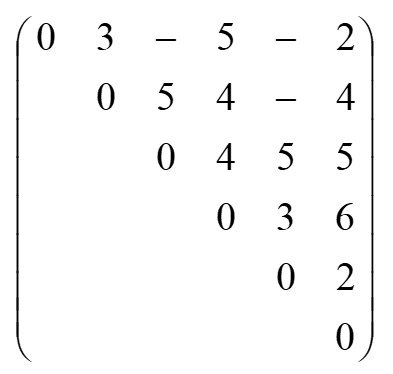
\includegraphics[width=0.5\textwidth]{pic/24.jpg}}
\end{minipage}
\end{figure}
